\qns{Transistor Switch Model}
\qcontributor{Ryan Koh}
\qcontributor{Son Tran}

Consider the circuit below, assume that when $t\leq0$, the capacitor has no charge stored $(V_{\text{c}}(t=0) = 0)$. At $t=0$, the switch closes. Assume that $V_s=\SI{5}{\volt}$, $R=\SI{100}{\ohm}$, and $C=\SI{10}{\micro\farad}$.

\begin{figure}[H]
	\begin{centering}
		\begin{circuitikz}
			\draw (0, 4)
			to[V =$V_s$] (0, 0);
			\draw (0, 4)
			to[switch,l^=\mbox{$t = 0$}](4,4)
			(4,4) to[R = $R$,v=$V_R(t)$,i>^=$i_R(t)$] (7,4)	
			to [short] (9,4)
			to[C = $C$, v=$V_C(t)$,i>^=$i_C(t)$] (9,0)
			to [short] (0,0);
		\end{circuitikz}
		\caption{\label{fig:circuit}RC Circuit with Voltage Source}
	\end{centering}
\end{figure}


\begin{enumerate}

\qitem Write out the KCL equations associated with the circuit when the switch is open. Then write out the differential equations for the case when the switch is closed.

\meta{
	Testing meta here
}

\sol{
\begin{align*}
\intertext{When the swtich is open, we denote the voltage to the left of resistor to be $y$. We obtain the following differential equations. KCL at node between the resistor and capacitor gives}
\frac{y - V_{\text{C}}}{R} = C\frac{dV_{\text{C}}}{dt} \\
\intertext{Since the current going into the resistor and the voltage source is zero, KCL gives:}
\frac{y - V_{\text{C}}}{R} = 0 \\
\intertext{and}
i_{\text{Vs}} = 0\\
\intertext{When the switch is closed, the following still holds:}
\frac{y - V_{\text{C}}}{R} = C\frac{dV_{\text{C}}}{dt} \\
\intertext{Additionally, KCL at the node between the resistor and voltage sources gives:}
\frac{V_{\text{S}} - V_{\text{C}}}{R} +  i_{\text{Vs}} = 0
\end{align*}
}



\qitem \textbf{Sketch the output voltage of the first inverter, showing clearly (1) the initial value, (2) the initial slope, (3) the asymptotic value, and (4) the time that it takes for the voltage to decay to roughly $\mathbf{\frac{1}{3}}$ of its initial value.}

\sol{
  (1) We know that the output of our inverter started with the initial value $V_{dd}$.

  (2) Since the differential equation tells us the change in value of $V_{out}(t)$ at time $t$ we can simply plug in $t = 0$ into our differential equation to get the initial slope:

  \begin{align*}
    \frac{d}{dt}V_{out}(t) = - \frac{V_{out}(0)}{R_{on}(C_{nmos} + C_{pmos})} \\
    \frac{d}{dt}V_{out}(t) = - \frac{V_{dd}}{R_{on}(C_{nmos} + C_{pmos})}
  \end{align*}

  Thus the initial slope is $\frac{V_{dd}}{R_{on}(C_{nmos} + C_{pmos})} = \frac{V_{dd}}{R_{on}(2C)}$

  (3) Since the input to the inverter changed from high to low we know the output of the inverter is going to go to $0$ in steady state.

  Another way to find this is: We know that the solution to a differential equation of the form $\frac{d}{dt}V_{out}(t) = - \frac{V_{out}}{R_{on}(C_{nmos} + C_{pmos})}$ is $V_{out} = ke^{-\frac{t}{R_{on}(2C)}}$.
  Plugging in the initial condition $V_{out}(0) = V_{dd}$ we find that $V_{out} = V_{dd}e^{-\frac{t}{R_{on}(2C)}}$.

  Plugging in $t = \infty$ we can see that the output approaches $V_{out} = V_{dd}e^{-\frac{\infty}{R_{on}(2C)}} = 0$.

  \begin{figure}[H]
  \begin{center}
    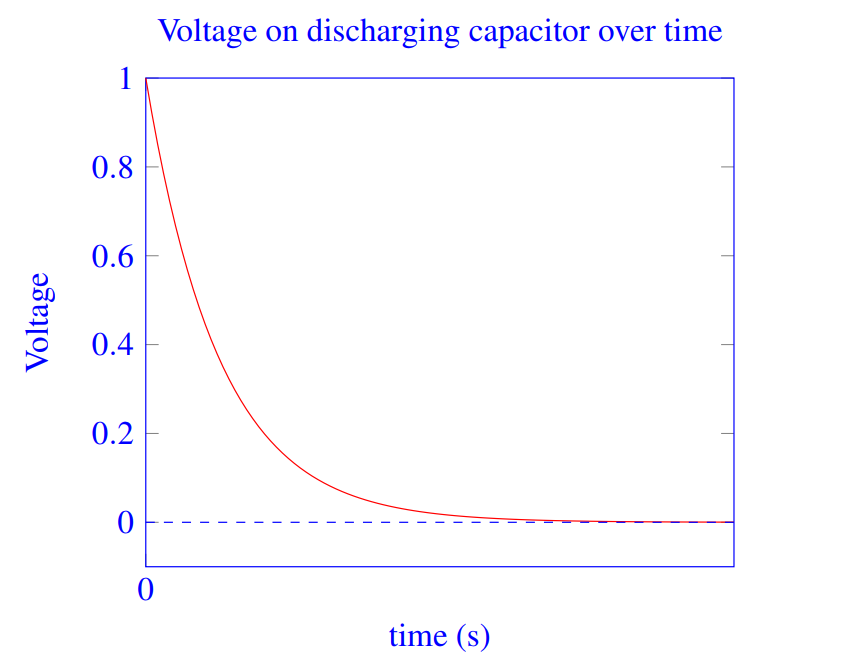
\includegraphics[width=0.6\linewidth]{\bank/ode/figures/discharging_capacitor.png}
  \end{center}
  \label{fig:discharging_capacitor}
\end{figure}


  (4) Using the fact that $e^{-1} = \frac{1}{e} \approx \frac{1}{3}$, we know that $V_{out} = V_{dd}e^{-1}$ which occurs when $t = R_{on}(2C) = 2 * 10^{-12}$.

  We know this from the solution $V_{out} = V_{dd}e^{-\frac{t}{R_{on}(2C)}}$ of the differential equation that we derived found in the previous part.
}



\qitem What is the initial condition for $V_{\text{c}}(t)$ (i.e. $V_{\text{c}}(t=0)$) and what is $V_{\text{c}}(t \to \infty)$?

\sol{

\begin{align*}
\intertext{No charge is on the capacitor before time $t=0$. Using $q=VC$, we know that $V_{\text{c}}=\SI{0}{\volt}$ before $t=0$.}
\intertext{At $t=0$, the switch closes. Since voltage across the capacitor cannot change instantaneously,}
V_{\text{c}}(t=0)&=0. \\
\intertext{As $t$ goes to infinity, the capacitor will become fully charged and the current goes to zero. Therefore, the voltage of the capacitor equals the voltage source:}
V_{\text{c}}(t \to \infty)&=V_{\text{S}}.
\end{align*}
}




\qitem Using the initial conditions found in the previous parts, find an expression for $V_{\text{c}}(t)$ in terms of $V_{\text{s}}$, $R$, and $C$.

\sol{
	\begin{align*}
		\intertext{The general solution to the equation}
		\frac{dy}{dt}&=\lambda y \\
		\intertext{is}
		y(t)&=Ke^{\lambda t}, \\
		\intertext{where $K$ is a constant and $\lambda$ is the eigenvalue of the equation. In our case, we know}
		C\frac{dV_{\text{C}}}{dt} + \frac{V_{\text{C}}}{R} - \frac{V_{\text{S}}}{R}=0,\\
		\intertext{which can be written as}
		\frac{dV_{\text{C}}}{dt} = - \frac{V_{\text{C}}}{RC} + \frac{V_{\text{S}}}{RC}.\\
		\intertext{The solution will be in the form}
		V_{\text{c}}(t)&=Ke^{-\frac{t}{RC}} + V_{\text{S}}. \\
		\intertext{To find $K$, we can plug in our initial condition at $t=0$:}
		V_{\text{c}}(t=0)&=K + V_{\text{S}} = 0.\\
		\intertext{So our overall equation ends up being}
		V_{\text{c}}(t)&=-V_{\text{S}} e^{-\frac{t}{RC}} + V_{\text{S}}. \\
		% % I_{\text{c}}(t=0)&=Ke^{-\frac{0}{RC}}=\frac{V_{\text{s}}}{R} \\
		% % \intertext{From this we can see}
		% % K&=\frac{V_{\text{s}}}{R} \\
		% % \intertext{So our overall equation ends up being}
		% % I_{\text{c}}(t)&=\frac{V_{\text{s}}}{R}e^{-\frac{t}{RC}} \\
		\intertext{We can also double check our answer by looking at the state for t $\to \infty$:}
		V_{\text{c}}(t \to \infty)&=-V_{\text{S}} e^{-\infty} + V_{\text{S}} =  V_{\text{S}},\\
		\intertext{which agrees with our answer from previous part.}
	\end{align*}
}

\qitem On what order of magnitude of time (nanoseconds, milliseconds, 10's of seconds, etc.) does this circuit settle ($V_{\text{c}}$ is $>95\%$ of its value as $t \to \infty$)?

\sol{

\begin{align*}
\intertext{The time constant $\tau$ of an RC circuit is just $\tau = RC$. For our circuit:}
\tau &= RC = \SI{100}{\ohm} \cdot \SI{10}{\micro\farad} = \SI{0.001}{\second} \\
\intertext{After 3 time constants, the voltage will be ~95\% of its steady state value}
3\tau &= \SI{0.003}{\second} \\
\intertext{The circuit will settle on the order of milliseconds.}
\end{align*}

}

\qitem Give 2 ways to reduce the settling time of the circuit if we are allowed to change one component in the circuit.

\sol{

To reduce settling time, reduce $\tau$. We can achieve this by

\begin{enumerate}
\item Lowering the value of $R$ or
\item Lowering the value of $C$.
\end{enumerate}

Notice how the value of $V_{\text{s}}$ does not change the settling time.

}


\end{enumerate}
